\nextchapter{Controllability and Observability}
\vspace{-2mm}
\begin{equation}\label{eq:gen_non_lin_sys}
\text{Consider general non-linear system: }
\arraycolsep=0pt
\begin{array}{rcl}
\dot x(t) & = & f(x(t),u(t),t) \\
y(t) & = & r(x(t),u(t),t)
\end{array}
\end{equation}
\begin{Definition}
$u(\cdot)\in PC([t_0,t_1],\Reals^m)$ \textbf{steers} $(x_0,t_0)$ to $(x_1,t_1)\Leftrightarrow s(t_1,t_0,x_0,u)=x_1$. System \textbf{controllable on $[t_0,t_1]$}$\Leftrightarrow\forall x_0,x_1\exists u(\cdot)\in PC([t_0,t_1],\Reals^m)$ that steers $(x_0,t_0)$ to $(x_1,t_1)$\mc{blue}{$\Leftrightarrow\forall x_0$, $s(t_1,t_0,x_0,\cdot)$ is surjective}.
\end{Definition}
\begin{minipage}{0.5\columnwidth}
\includegraphics[width=1\columnwidth]{figures/state_output_feedback.pdf}
\end{minipage}%
\begin{minipage}{0.5\columnwidth}
\begin{itemize}[leftmargin=4mm]
  \item Open loop: $\dot x=f(x,u,t)$
  \item State feedback: $\dot x=f(x,v+F_S(x,t),t)=f_S(x,v,t)$
  \item Output feedback: $\dot x=f(x,w+F_O(y,t),t)=f_O(x,w,t)$
  \item Input feedforward: $z(t)=r(x,u,t)+F_F(u,t)=r_F(x,u,t)$
\end{itemize}
\begin{Theorem}
Controllable on $[t_0,t_1]$ open loop$\Leftrightarrow$state feedb.$\Leftrightarrow$output feedb.
\end{Theorem}
\end{minipage}
\begin{Definition}
System (\ref{eq:gen_non_lin_sys}) \textbf{observable on $[t_0,t_1]$}$\Leftrightarrow\forall x_0\in\Reals^n,\forall u(\cdot)\in PC([t_0,t_1],\Reals^m)$, given $u(t\in [t_0,t_1])$ and corresp. $y(t\in [t_0,t_1])$, the val. of $x_0$ can be uniquely determined\mc{blue}{$\Leftrightarrow\forall u(\cdot)\in PC([t_0,t_1],\Reals^m), \rho(\cdot,t_0,\odot,u):x_0\mapsto \rho(\cdot,t_0,x_0,u):[t_0,t_1]\to\Reals^p$ is injective.}
\end{Definition}
NB: once $x_0$ known, $x(t)=s(t,t_0,x_0,u)$ uniquely established!

\begin{Theorem}
Observable on $[t_0,t_1]$ open loop$\Leftrightarrow$output feedb.$\Leftrightarrow$input feedf.
\end{Theorem}
\nextsubchapter{LTV Controllability (abbreviation: ctrb.)}
\begin{Definition}
$(A(\cdot),B(\cdot))$ \textbf{controllable on $[t_0,t_1]$}$\Leftrightarrow\forall x_0,x_1\in\Reals^n\exists u:[t_0,t_1]\to\Reals^m$ that steers $(x_0,t_0)$ to $(x_1,t_1)$: $x_1=\Phi(t_1,t_0)x_0+\int_{t_0}^{t_1}\Phi(t_1,\tau)B(\tau)u(\tau)d\tau$.
\end{Definition}
\begin{Theorem}
\hl{Equivalent}: \begin{itemize*}
\item $(A(\cdot),B(\cdot))$ \mc{blue}{controllable} on $[t_0,t_1]$
\item $\forall x_0\exists u$ steering $(x_0,t_0)$ to $(0,t_1)$ (\mc{blue}{controllability to 0})
\item $\forall x_1\exists u$ steering $(0,t_0)$ to $(x_1,t_1)$ (\mc{blue}{reachability from 0})
\end{itemize*}
\end{Theorem}
\begin{Definition}
$x_1$ \textbf{reachable on $[t_0,t_1]$}$\Leftrightarrow\exists u(\cdot)\in L^2$ steering $(0,t_0)\to (x_1,t_1)$. \textbf{Reachability map on $[t_0,t_1]$} of $(A(\cdot),B(\cdot))$ is \hl{$\mathcal L_r(u)=\int_{t_0}^{t_1}\Phi(t_1,\tau)B(\tau)u(\tau)d\tau:L^2([t_0,t_1],\Reals^m)\to\Reals^n$}, \mc{blue}{linear \& continuous}! $\Range(\mathcal L_r):=$ \textbf{set of reachable states}! Since $\mathcal L_r:L^2([t_0,t_1],\Reals^m)\to\Reals^n$ Hilbert spaces, \textit{can apply \hyperlink{FRL}{FRL}}!
\end{Definition}
\begin{Definition}
\textbf{Controllability Gramian} of $(A(\cdot),B(\cdot))$ on $[t_0,t_1]$: \hl{$W_r(t_0,t_1)=\int_{t_0}^{t_1}\Phi(t_1,\tau)B(\tau)B(\tau)^T\Phi(t_1,\tau)^Td\tau\in\Reals^{n\times n}$}, it's the matrix rep. of $\mathcal L_r\circ\mathcal L_r^*:\Reals^n\to\Reals^n$. \textit{Use to analyze LTV ctrblty}!

\begin{Fact}
$W_r(t_0,t_1)$ is symmetric, positive semidefinite and $\forall t_0'\le t_0,\mc{red}{W_r(t_0',t_1)}\ge W_r(t_0,t_1)$ (``\mc{red}{\hl{\textit{less} effort req when more time available}}''), i.e. $x^T[W_r(t_0',t_1)-W_r(t_0,t_1)]x\ge 0\forall x\in\Reals^n$
\end{Fact}
\end{Definition}
\begin{Theorem}
$(A(\cdot),B(\cdot))$ controllable on $[t_0,t_1]$ $\Leftrightarrow$ $\Range(\mathcal L_r)=\Reals^n$ $\Leftrightarrow$ $\Range(\mathcal L_r\circ\mathcal L_r^*)=\Reals^n$ $\Leftrightarrow$ $\Det[W_r(t_0,t_1)]\ne 0$ (\mc{blue}{otherwise $=0$}).
\end{Theorem}
\nextsubchapter{LTV Minimum Energy Control}
\begin{minipage}{0.2\columnwidth}
\begin{turn}{90}
\includegraphics[height=1\columnwidth]{figures/lin_space_decomposition_reachability.pdf}
\end{turn}
\end{minipage}%
\begin{minipage}{0.8\columnwidth}
Idea: $\widetilde u\in\Range(\mathcal L_r^*)$ is the unique input 2-norm minimizer (cf. \hyperlink{min_theorem7_3}{\textbf{\mc{blue}{($\blacksquare$)}}}).
\begin{Theorem}
$(A(\cdot),B(\cdot))$ controllable on $[t_0,t_1]$. Given $x_0,x_1\in\Reals^n$, define:
\begin{equation*}
\arraycolsep=0pt
\begin{array}{rcl}
\widetilde u(t) & = & 
\mathcal L_r^*\circ(\mathcal L_r\circ\mathcal L_r^*)^{-1}[x_1-\Phi(t_1,t_0)x_0] \\
& = & B(t)^T\Phi(t_1,t)^TW_r(t_0,t_1)^{-1}[x_1 \\
& & -\Phi(t_1,t_0)x_0]\quad\forall t\in[t_0,t_1]
\end{array}
\end{equation*}
\begin{enumerate}[leftmargin=4mm]
  \item $\widetilde u$ steers $(x_0,t_0)\to (x_1,t_1)$
  \item $\widetilde u$ pwc w/ discont. set of $B(\cdot)$. $\widetilde u$ cont.$\Leftrightarrow B(\cdot)$ cont.
  \item $\fnorm{\widetilde u}{2}^2=[x_1-\Phi(t_1,t_0)x_0]^T W_r(t_0,t_1)^{-1}[x_1-\Phi(t_1,t_0)x_0]$
  \item If $u$ steers $(x_0,t_0)\to (x_1,t_1)\Rightarrow\fnorm{u}{2}\ge\fnorm{\widetilde u}{2}$
\end{enumerate}
\end{Theorem}
\end{minipage}
\begin{Fact}
From 3.: $\fnorm{\widetilde u}{2}^2\propto W_r(t_0,t_1)^{-1}\Rightarrow$ the ``smaller'' (i.e. more singular) $W_r(t_0,t_1)$, the ``more energy'' needed to steer to $(x_1,t_1)$.
\end{Fact}
\nextsubchapter{LTV Observability and Duality (abbreviation: obsvb.)}
\begin{Definition}
$(C(\cdot),A(\cdot))$ \textbf{observable on $[t_0,t_1]$}$\Leftrightarrow\forall x_0\in\Reals^n,\forall u:[t_0,t_1]\to\Reals^m$ can uniquely determine $x_0$ from $\{(u(t),y(t))|t\in [t_0,t_1]\}$.
\end{Definition}
\begin{Definition}
$x_0$ \textbf{unobservable on $[t_0,t_1]$}$\Leftrightarrow C(t)\Phi(t,t_0)x_0=0\forall t\in[t_0,t_1]\Leftrightarrow x_0\in\Null(\mathcal L_o)$ \textbf{observability map} \hl{$\mathcal L_o=C(t)\Phi(t,t_0)x_0:\Reals^n\to L^2([t_0,t_1],\Reals^p)$} with $\Range(\mathcal L_o)=PC([t_0,t_1],\Reals^p)$ w/ discont. set of $C(\cdot)$.
\end{Definition}
\begin{Fact}
Consequence: $x_0=0$ is unobservable!
\end{Fact}
\begin{Definition}
\textbf{Observability Gramian} of $(C(\cdot),A(\cdot))$ on $[t_0,t_1]$: \hl{$W_o(t_0,t_1)=\int_{t_0}^{t_1}\Phi(\tau,t_0)^TC(\tau)^TC(\tau)\Phi(\tau,t_0)d\tau\in\Reals^{n\times n}$}, it's the matrix rep. of $\mathcal L_o^*\circ\mathcal L_o:\Reals^n\to\Reals^n$.
\end{Definition}
\begin{Theorem}
$(C(\cdot),A(\cdot))$ observable on $[t_0,t_1]\Leftrightarrow\Null(\mathcal L_o)=\{0\}\Leftrightarrow\Null(\mathcal L_o^*\circ\mathcal L_o)=\{0\}\Leftrightarrow\Det[W_o(t_0,t_1)]\ne 0$ (\mc{blue}{otherwise $=0$}).
\end{Theorem}
\begin{minipage}{0.2\columnwidth}
\begin{turn}{90}
\includegraphics[height=1\columnwidth]{figures/lin_space_decomposition_observability.pdf}
\end{turn}
\end{minipage}%
\begin{minipage}{0.8\columnwidth}
Let $\circled{1}\begin{cases}
\dot x=Ax+Bu \\
y=Cx+Du
\end{cases}\circled{2}\begin{cases}
\dot{\overline x}=-A^T\overline x-C^T\overline u \\
\overline y=B^T\overline x+D^T\overline u
\end{cases}$

\begin{Theorem}
\circled{1} (w/ state. trans. mat. $\Phi(t,t_0)$) and \circled{2} (w/ state. trans. mat. $\Psi(t,t_0)$) ($t$ ommitted) have:
\begin{itemize}[leftmargin=3mm]
  \item \hspace{-1mm}$\Psi(t,t_0)=\Phi(t_0,t)^T$ (solve $\dot X(t)=-A(t)^TX(t)$)
  \item \hspace{-1mm}\circled{1} ctrb. on $[t_0,t_1]\Leftrightarrow\circled{2}$ obsvb. on $[t_0,t_1]$.
  \item \hspace{-1mm}\circled{1} obsvb. on $[t_0,t_1]\Leftrightarrow\circled{2}$ ctrb. on $[t_0,t_1]$.
\end{itemize}
\end{Theorem}
\begin{Theorem}
$(C(\cdot),A(\cdot))$ observable on $[t_0,t_1]$. Given $y\in L^2([t_0,t_1],\Reals^p)$, define:
\begin{equation*}
\arraycolsep=0pt
\begin{array}{rcl}
x_0 & = &
(\mathcal L_o^*\circ\mathcal L_o)^{-1}\circ\mathcal L_o^*(y) \\
& = &
[W_o(t_0,t_1)]^{-1}\int_{t_0}^{t_1}\Phi(\tau,t_0)^TC(\tau)^Ty(\tau)d\tau
\end{array}
\end{equation*}
\end{Theorem}
\end{minipage}
\vspace{-0.5mm}
\begin{Theorem}
$x_0$ is the unique minimizer of $\fnorm{y-\mathcal L_o(x)}{2}$ over $x\in\Reals^n$ w/ $\min_{x\in\Reals^n}\fnorm{y-\mathcal L_0(x)}{2}^2=\fnorm{y}{2}^2-x_0^TW_o(t_0,t_1)x_0$
\end{Theorem}



\nextsubchapter{LTI Observability}
\begin{Definition}
\textbf{\hl{Observability matrix}}: $O=[C;CA;\cdots;CA^{n-1}]\in\Reals^{pn\times n}$.
\end{Definition}
\begin{Theorem}
\begin{itemize}[leftmargin=3mm]
  \item \hspace{-1.5mm}\hl{$\Null(O)=\Null(\mathcal L_o)=\{x_0\in\Reals^n | \text{unobservable}\}$}
  \item \hspace{-1.5mm}$\Null(O)$ is $A$ invariant subspace,$\therefore x\in\Null(O)\Rightarrow Ax\in\Null(O)$
\end{itemize}
\end{Theorem}
\begin{Theorem}
$\forall [t_0,t_1]$, $(C,A)$ observable on $[t_0,t_1]\Leftrightarrow\Rank(O)=n\Leftrightarrow\forall\lambda\in\Spec[A],\Rank([\lambda I-A;C]\in\Reals^{(n+p)\times n})=n$ (\texttt{MATLAB notation!}).
\end{Theorem}
\begin{Corollary}
$(C,A)$ observable on some $[t_0,t_1]\Leftrightarrow$ observable $\forall [t_0,t_1]$.
\end{Corollary}
\begin{Theorem}
$\forall C\in\Reals^{p\times r},A\in\Reals^{n\times n}\exists T\in\Reals^{n\times n}, \Det[T]\ne 0$ s.t. in this basis the matrices decompose into:
\begin{equation*}
\widehat A=TAT^{-1}=\begin{bmatrix}
A_{11} & 0 \\
A_{21} & A_{22}
\end{bmatrix}
\qquad\widehat C=CT^{-1}=\begin{bmatrix}
C_1 & 0
\end{bmatrix}
\end{equation*}
and the pair of matrices $(C_1,A_{11})$ is \textbf{observable}!

\begin{Method}
FRL: $\Reals^n=\Null(O)\overset{\perp}{\oplus}\Null(O)^\perp=\Null(O)\overset{\perp}{\oplus}\Range(O^T)$. So:
\begin{enumerate}[label=\protect\circled{\arabic*},leftmargin=4mm]
  \item New $\Reals^n$ basis $\basis{y}{i}{n}=\{w_1,\ldots,w_{n-r},v_1,\ldots,v_r\}$
  
  \begin{itemize*}
    \item $\basis{v}{i}{r}$ basis of $\Null(O)$.
  \item $\basis{w}{i}{n-r}$ basis of $\Range(O^T)$.
  \end{itemize*}
  \item $T=$ transf mat $\{e_i\}\to\{y_i\}$ (where $\{e_i\}$ canonical basis). So:
  $T^{-1}=[w_1,\ldots,w_{n-r},v_1,\ldots,v_r]$ simply!
\end{enumerate}
\end{Method}
\begin{Definition}
NB: $\Spec[A]\equiv\Spec[\widehat A]=\Spec[A_{11}]\union\Spec[A_{22}]$ where $\Spec[A_{11}]$ contains eigvals whose eigvecs obsvb. (\textbf{obsvb. modes}), $\Spec[A_{22}]$ eigevals whose eigvecs unobsvb. (\textbf{unobsvb. modes}).
\end{Definition}
\end{Theorem}
Danger of unobservability: an unobservable mode may diverge $\to\infty$ if unstable, yet no indication at output!

\begin{Definition}
If all unobservable modes are stable, system \textbf{detectable}.
\end{Definition}




\nextsubchapter{LTI Controllability}
\begin{Definition}
\textbf{\hl{Controllability matrix}}: $P=[B,AB,\cdots ,A^{n-1}B]\in\Reals^{n\times{nm}}$.
\end{Definition}
\begin{Theorem}
\begin{itemize}[leftmargin=3mm]
  \item \hspace{-1.5mm}\hl{$\Range(P)=\Range(\mathcal L_r)=\{x_1\in\Reals^n | \text{reachable}\}$}
  \item \hspace{-1.5mm}$\Range(P)$ is an $A$ invariant subspace
\end{itemize}
\end{Theorem}
\begin{Theorem}
$\forall [t_0,t_1]$, $(A,B)$ controllable on $[t_0,t_1]\Leftrightarrow\Rank(P)=n\Leftrightarrow\forall\lambda\in\Spec[A],\Rank([\lambda I-A,B]\in\Reals^{n\times(n+m)})=n$ (\texttt{MATLAB notation!}).
\end{Theorem}
\begin{Theorem}
$\forall B\in\Reals^{n\times m},A\in\Reals^{n\times n}\exists T\in\Reals^{n\times n}, \Det[T]\ne 0$ s.t. in this basis:
\begin{equation*}
\widehat A=TAT^{-1}=\begin{bmatrix}
A_{11} & A_{12} \\
0      & A_{22}
\end{bmatrix}
\qquad\widehat B=TB=\begin{bmatrix}
B_1 \\ 0
\end{bmatrix}
\end{equation*}
and the pair of matrices $(A_{11},B_1)$ is \textbf{controllable}!

\begin{Method}
FRL: $\Reals^n=\Range(P)\overset{\perp}{\oplus}\Range(P)^\perp=\Range(P)\overset{\perp}{\oplus}\Null(P^T)$. So:
\begin{enumerate}[label=\protect\circled{\arabic*},leftmargin=4mm]
  \item New $\Reals^n$ basis $\basis{y}{i}{n}=\{v_1,\ldots,v_r,w_1,\ldots,w_{n-r}\}$
  
  \begin{itemize*}
    \item $\basis{v}{i}{r}$ basis of $\Range(P)$.
  \item $\basis{w}{i}{n-r}$ basis of $\Null(P^T)$.
  \end{itemize*}
  \item $T=$ transf mat $\{e_i\}\to\{y_i\}$ (where $\{e_i\}$ canonical basis). So:
  $T^{-1}=[v_1,\ldots,v_r,w_1,\ldots,w_{n-r}]$ simply!
\end{enumerate}
\end{Method}
\begin{Definition}
NB: $\Spec[A]\equiv\Spec[\widehat A]=\Spec[A_{11}]\union\Spec[A_{22}]$ where $\Spec[A_{11}]$ contains eigvals whose eigvecs reachable (\textbf{ctrb. modes}), $\Spec[A_{22}]$ eigvals whose eigvecs unreachable (\textbf{unctrb. modes}).
\end{Definition}
\end{Theorem}
\begin{Definition}
If all uncontrollable modes are stable, system \textbf{stabilizable}.
\end{Definition}